
\chapter{Data types}

\section{Identifiers and keywords}

The name we give to our object references are called \keyword{identifiers} or just plain \keyword{names}.



A valid Python identifier is a \keyword{nonempty} sequence of characters of any length that consists of a ``start character'' and zero or more ``continuation characters''.
Such an identifier must obey a couple of rules and ought to follow certain conventions.


Rules:
\begin{itemize}
\item The start character can be anything that Unicode considers to be a letter.
\item Each continuation character can be any character that is permitted as a start character, or any nonwhitespace character.
\item No identifier can have the same name as one of Python's keywords.
\end{itemize}


Python has a built-in function called \verb|dir()| that returns a list of object's attributes.


Conventions:
\begin{itemize}
\item Don't use the name of any of Python's predefined identifiers for your own identifiers.
\item Names that begin and end with two underscores should not be used.
\end{itemize}


\section{Integral types}

Python provides two built-in integral types, \verb|int| and \verb|bool|.
Both integers and Boolean are imuutable.
When used in Boolean expressions, 0 and \verb|False| are \verb|False| and any other integer and \verb|True| are \verb|True|.
When used in numerical expressions \verb|True| evaluates to 1 and \verb|False| to 0.



\subsection{Integers}

Integer literals are written using base 10 by default, but other number bases can be used.

\begin{lstlisting}

>>> 14600926                      # decimal
14600926
>>> 0b110111101100101011011110    # binary
14600926                          
>>> 0o67545336                    # octal
14600926
>>> 0xDECADE                      # hexadecimal
14600926
\end{lstlisting}



Binary numbers are written with a leading \verb|0b|,
octal numbers with a leading \verb|0o|, and
hexadecimal numbers with a leading \verb|0x|.
Uppercase letters can also be used.



All the usual mathematical functions and operators can be used with integers.
Some of the functionality is provided by functions and other functionality is provided by \verb|int| operators.


Provided by operators:
\begin{description}
\item[x + y] 
\item[x - y]
\item[x * y] 
\item[x / y] Divdes $x$ by $y$; always produces a \verb|float| (or a \verb|complex| if $x$ or $y$ is \verb|complex|)
\item[x // y] Divdes $x$ by $y$; truncates any fractional part so always produces an \verb|int| result
\item[x \% y]   
\item[x ** y] Same to $x^y$
\item[-x] Negates x;
\item[+x] Does nothing; is sometimes used to clarify code
\item[x | y] Bitwise \verb|OR| 
\item[x \^{} y] Bitwise \verb|XOR|
\item[x \&{} y|] Bitwise \verb|AND|
\item[i $>>$ j] Shifts \verb|i| left by \verb|j|; like \verb|i * (2 ** j)| without overflow checking
\item[i $<<$ j] Shifts \verb|i| right by \verb|j|; like \verb|i // (2 ** j)| without overflow checking
\item[\~{}i]  Inverts \verb|i|'s bits
\end{description}

Provided by functions:
\begin{description}
\item[abs(x)] Return the absolute value of $x$
\item[divmod(x, y)] Return the quotient and remaninder of dividing $x$ by $y$ as a tuple of two \verb|int|s
\item[pow(x, y)] Same to $x^y$
\item[pow(x, y, z)] A faster alternative to $(x ** y) \% z$
\item[round(x, n)] Return $x$ rounded to $n$ integral digits if $n$ is a negative \verb|int| or return $x$ rounded to $n$ decimal places if $n$ is a positive \verb|int|; the returned value has the same type as x;
\item[bin(i)] Return the binary representation of \verb|int i| as a string
\item[hex(i)] 
\item[int(x)] Convert object $x$ to an integer
\item[int(s, base)] Convert \verb|str s| to an integer. \verb|base| should be an integer between 2 and 36 inclusive.
\item[oct(i)] 
\end{description}



All the binary numeric operators (+, -, /, //, \%, and **) have augmented assignment versions (+=, -=, /=, //=, \%=, and **=) where \verb|x op= y| is logically equivalent to \verb|x = x op y| in the normal case when reading x’s value has no side effects.

All the binary bitwise operators (|, \^{}, \&{}, $<<$, and $>>$) have augmented assignment versions (|=, \^{}=, \&{}=, $<<=$, and $>>=$) where \verb|i op= j| is logically equivalent to \verb|i = i op j| in the normal case when reading \verb|i|’s value has no side effects.


\begin{tcolorbox}
When an object is created using its data types there are 3 possible use cases:
\begin{enumerate}
\item When a data type is called with no arguments an object with a default value is created.
\item When the data type is called with a sinle argument, if an argument of the same type is given, a new object which is a shallow copy of the original object is created. If argument of a different type is given, a conversion is attempted.
\item If two or more arguments are given --- not all types support this, and for those that do the argument types and their meanings vary.
\end{enumerate}
\end{tcolorbox}


\subsection{Booleans}

There are two built-in Boolean objects: \verb|True| and \verb|False|.

\section{Floating-point types}

Python provides three kinds of floating-point values:
\begin{itemize}
\item the built-in \verb|float|
\item the built-in \verb|complex|
\item the \verb|decimal.Decimal| type from the standard library
\end{itemize}
All three are immutable.


\verb|decimal.Decimal| perform calculations that are accurate to the level of precision we specify (by default, to 28 decimal places) and can represent periodic numbers like 0.1 exactly; but processing is a lot slower than with \verb|float|s.
Because of their accuracy, \verb|decimal.Decimal| numbers are suitable for financial calculations.



\subsection{Floating-point numbers}

\begin{tcolorbox}
  \begin{lstlisting}

import sys

# the samllest difference that the machine can distinguish 
# between two floating-point numbers
sys.float_info.epsilon 

help(sys.float_info)
  \end{lstlisting}
\end{tcolorbox}

The \verb|math| module provides many functions that operate on \verb|float|s.
The \verb|math| module is very dependent on the underlying math library that Python was compiled against.
This means that some error conditions and boundary cases may behave differently on different platforms.


\begin{description}
\item[math.copysign(x, y)] Returns \verb|x| with \verb|y|'s sign
\item[math.e] 
\item[math.pi] 
\item[math.exp(x)] 
\item[math.factorial(x)] Returns $x!$
\item[math.floor(x)] 
\item[math.ceil(x)] 
\item[math.hypot(x, y)] Returns $\sqrt(x^2 + y^2)$
\item[math.isinf(x)] Returns \verb|True| if \verb|float x| is $\pm \mathrm{inf}(\pm \infty)$
\item[math.isnan(x)] Returns \verb|True| if \verb|float x| is nan (``not a number'')
\item[math.log(x, b)] Returns $\log_bx$
\item[math.log10(x)] Returns $\log_{10}x$
\item[math.sqrt(x)] 
\end{description}




\subsection{Complex numbers}

The \verb|complex| data type is an immutable type that holds a pair of \verb|float|s, one representing the real part and the other the imaginary part of a complex number. 

\begin{lstlisting}

>>> z = 1.0 + 2.0j
>>> z.real, z.imag
(1.0, 2.0)
\end{lstlisting}



The functions in the \verb|math| module do not work with complex numbers while \verb|cmath| module does.



\subsection{Decimal numbers}

\begin{lstlisting}

>>> import decimal
>>> a = decimal.Decimal(1234)
>>> b = decimal.Decimal('54321.012345678987654321')
>>> a + b
Decimal('55555.012345678987654321')
\end{lstlisting}



Numbers of type \verb|decimal.Decimal| work within the scope of a \keyword{context}; the context is a collection of settings that affect how \verb|decimal.Decimal| behave.


\begin{lstlisting}

>>> 23 / 1.05
21.904761904761905
>>> print(23 / 1.05)
21.904761904761905
>>> print(decimal.Decimal(23) / decimal.Decimal(1.05))
21.90476190476190383546015179
>>> decimal.Decimal(23) / decimal.Decimal(1.05)
Decimal('21.90476190476190383546015179')
\end{lstlisting}


When we call \verb|print()| on the result of \\
\verb|decimal.Decimal(23) / decimal.Decimal(1.05)| the bare number is printed --- this output is in \keyword{string form}.
If we simply enter the expression we get a \verb|decimal.Decimal| output --- this output is in \keyword{representational form}.
All Python objects have two output forms. String form is designed to be human-readable. Representational form is designed to produce output that if fed to a Python interpreter would (when possible) reproduce the represented object.



\section{Strings}

Strings are represented by the immutable \verb|str| data type which holds a sequence of Unicode characters.

triple quoted string: 
\begin{lstlisting}

text = """hello world"""
\end{lstlisting}


\begin{tcolorbox}
Python uses newline as its \keyword{statement terminator}, except inside parentheses (()), square brackets ([]), braces ({}), or triple quoted strings.  
\end{tcolorbox}


All of Python's escape sequences are shown in Table \ref{fig:escapes}.

\begin{figure}[!ht]
  \centering
  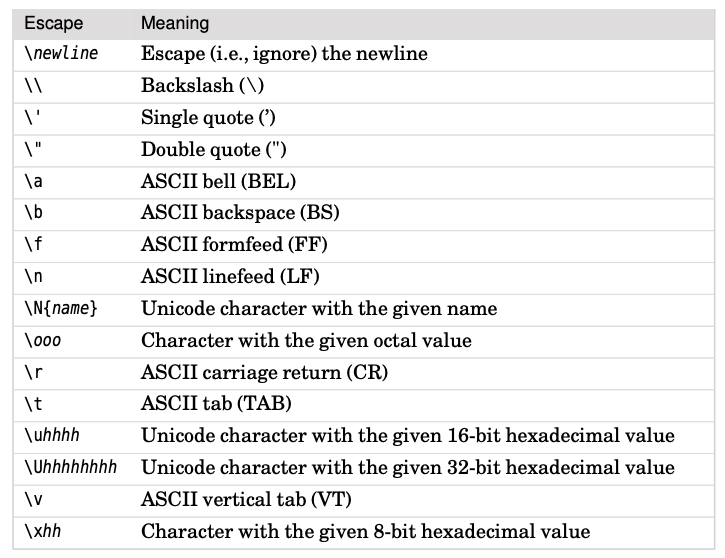
\includegraphics[width=\textwidth]{pics/escapes}
  \caption{Python's string escapes }
  \label{fig:escapes}
\end{figure}

In some situations --- for example, when writing regular expressions --- we need to create strings with lots of literal backslashes.
This can be inconvenient since each one must be escaped:
\begin{lstlisting}

import re
phone1 = re.compile("^((?:[(]\\d+[)])?\\s*\\d+(?:-\\d+)?)$")
\end{lstlisting}


The solution is to use \keyword{raw} strings.
These are quoted or triple quoted strings whose first quote is preceded by the letter \verb|r|.
Inside such strings all characters are taken to be literals, so no escaping is necessary.

\begin{lstlisting}

phone2 = re.compile(r"^((?:[(]\d+[)])?\s*\d+(?:-\d+)?)$")
\end{lstlisting}



\begin{lstlisting}

>>>'\N{euro sign}'
'€'
\end{lstlisting}



If we want to know the Unicode code point for a particular character in a string, we can use the built-in \verb|ord()| function:
\begin{lstlisting}

>>> ord('€')
8364
>>> hex(ord('€'))
'0x20ac'
>>> '\u20ac'
'€'
\end{lstlisting}


we can convert any integer that represents a valid code point into the corresponding Unicode character using the built-in \verb|chr()| function:

\begin{lstlisting}

>>> chr(8734)
'∞'
>>> chr(8364)
'€'
>>> ascii('€')
"'\\u20ac'"
\end{lstlisting}



\subsection{Comparing strings}

Strings support the usual comparison operators <, <=, ==, !=, >, and >=.
These operators compare strings byte by byte in memory.

\subsection{Slicing and striding strings}

\begin{lstlisting}

s = "Light ray"
\end{lstlisting}

Figure \ref{fig:string-index-position} shows all the valid index postions for string \verb|s|.

\begin{figure}[!ht]
  \centering
  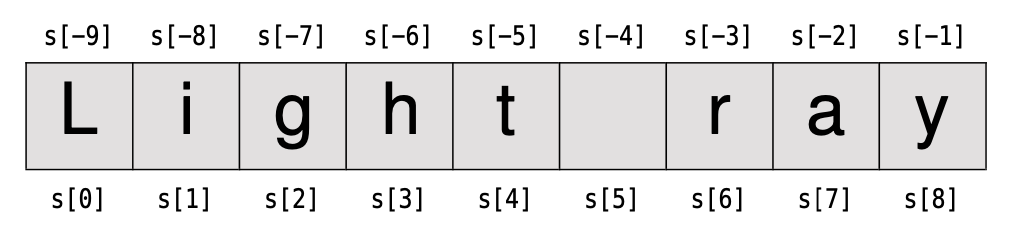
\includegraphics[width=\textwidth]{pics/string-index-position}
  \caption{String index position}
  \label{fig:string-index-position}
\end{figure}

The slice operator has three syntaxes:
\begin{verbatim}
seq[start]
seq[start:end]
seq[start:end:step]
\end{verbatim}


Using \verb|+| to concatenate and \verb|+=| to append is not particularly efficient when String
many strings are involved.
For joining lots of strings it is usually best to use the \verb|str.join()| method.



\subsection{String operators and methods}

Since strings are immutable sequences, all the functionality that can be used with imuutable sequences can be used with strings.

\begin{itemize}
\item membership (in)
\item concatenation (+)
\item appedning (+=)
\item replication (*)
\item augmented assignment replication (*=)
\end{itemize}


There are some common string methods:
\begin{description}
\item[s.capitalize()] 
\item[s.lower()] 
\item[s.title()] 
\item[s.upper()] 
\item[s.swapcase()] 
\item[s.center(width, char)]
\item[s.ljust(width, char)] 
\item[s.rjust(width, char)] 
\item[s.count(t, start, end)] 
\item[s.encode(encoding, err)] 
\item[s.startswith(x, start, end)] 
\item[s.endswith(x, start, end)] 
\item[s.expandtabs(size)] 
\item[s.find(t, start, end)] 
\item[s.index(t, start, end)] 
\item[s.format(...)] 
\item[s.isalnum()] 
\item[s.isalpha()] 
\item[s.isdecimal()] 
\item[s.isdigit()] 
\item[s.isidentifier()] 
\item[s.islower()]
\item[s.istitle()] 
\item[s.isupper()] 
\item[s.isnumeric()] 
\item[s.isprintable()] 
\item[s.isspace()] 
\item[s.join(seq)] 
\item[s.partition(t)] 
\item[s.replace(t, u, n)] 
\item[s.split(t, n)] 
\item[s.splitlines(f)] 
\item[s.strip(chars)] 
\item[s.maketrans()] 
\item[s.translate()] 
\item[s.zfill(w)] 
\end{description}

\subsection{String formatting with the str.format() method}

The \verb|str.format()| method returns a new string with the replacement fields in its string replaced with its arguments suitablely formatted.


\begin{lstlisting}

>>> "{0} {1} {2}".format("Hello", 'world', 'mike')
'Hello world mike'
\end{lstlisting}


Each replacement field is identified by a field name in braces.
If the field name is a simple integer, it is taken to be the index position of one of the arguments passed to \verb|str.format()|.


If we need to include braces inside format strings, we can do so by doubling them up.
\begin{lstlisting}

>>> 'just {{{0}}}'.format('brace')
'just {brace}'
\end{lstlisting}



The replacement field can have any of the following general syntaxes:
\begin{verbatim}
{field_name}
{field_name!conversion}
{field_name:format_specification}
{field_name!conversion:format_specification}
\end{verbatim}


\subsection{Field names}

A field name can be either an integer corresponding to one of the \verb|str.format()| method’s arguments, or the name of one of the method’s keyword arguments.

\begin{lstlisting}

>>> '{who} solve a leetcode problem every {0} days'.format(1, who='Mike')
'Mike solve a leetcode problem every 1 days'
\end{lstlisting}


Notice that in an argument list, keyword arguments always come after positional arguments.



If the arguments are collections data types like lists or dictionaries, or have attributes, we can access the part using [] or . notation.


\begin{lstlisting}

>>> stock = ["paper", "envelopes", "notepads"] 
>>> "We have {0[1]} and {0[2]} in stock".format(stock)
'We have envelopes and notepads in stock'

>>> d = dict(animal="elephant", weight=12000)
>>> "The {0[animal]} weighs {0[weight]}kg".format(d) 
'The elephant weighs 12000kg'

>>> "math.pi=={0.pi}".format(math) 
'math.pi==3.14159265359
\end{lstlisting}




The local variables that are currently in scope are available from the built-in \verb|locals()| function.
This function returns a dictionary whose keys are local variable names and whose values are references to the variables' values.
We can use \keyword{mapping unpacking} to feed this dictionary into the \verb|str.format()| method.
The mapping unpacking operator is \verb|**| and it can be applied to a mapping (such as dictionary) to produce a key-value list suitable for passing to a function.
For example:
\begin{lstlisting}

>>> element = "Silver"
>>> number = 47
>>> "Element {number} is {element}".format(**locals()) 
'Element 47 is Silver'
\end{lstlisting}




\subsection{conversions}

\begin{lstlisting}

>>> decimal.Decimal("3.4084") 
Decimal('3.4084')
>>> print(decimal.Decimal("3.4084")) 
3.4084
\end{lstlisting}


The first is in representational form.
The purpose of this form is to provide a string which if interpreted by Python would re-create the ojbect it represents.
Not all objects can provide a reproducing representation, in which case they provide a string enclosed in angle brackets.
For example \verb|"module 'sys' (built-in)>"|.

The second is in its string form.
This form is aimed at human readers, so the concern is to show something that makes sense to people.
If a data type doesn’t have a string form and a string is required, Python will use the representational form.


Python’s built-in data types know about \verb|str.format()|, and when passed as an argument to this method they return a suitable string to display themselves.
In addition, it is possible to override the data type’s normal behavior and force it to provide either its string or its representational form.
This is done by adding a conversion specifier to the field.
Currently there are three such specifiers:
\begin{itemize}
\item \verb|s| to force string form, 
\item \verb|r| to force representational for
\item \verb|a| to for representational form but only using ASCII characters.
\end{itemize}


\begin{lstlisting}

>>> "{0}  {0!s}  {0!r}  {0!a}  {1!r}  {1!a}".format(decimal.Decimal(1), "你好")
"1  1  Decimal('1')  Decimal('1')  '你好'  '\\u4f60\\u597d'"
\end{lstlisting}



\subsection{Format specifications}

\subsubsection{Specification for string}

For strings, the things that we can control are:
\begin{itemize}
\item the fill character, 
\item the alignment within the field, and 
\item the minimum and 
\item maximum field widths.
\end{itemize}

\begin{tcolorbox}
\begin{verbatim}
: fill     align        min_width   .max_width
            < for left
            > for right
            ^ for center
\end{verbatim}
\end{tcolorbox}


\begin{lstlisting}

>>> s = "The sword of truth"
>>> '{0}'.format(s)
'The sword of truth'
>>> '{0:25}'.format(s)
'The sword of truth       '
>>> '{0:>25}'.format(s)
'       The sword of truth'
>>> '{0:->25}'.format(s)
'-------The sword of truth'
>>> '{0:.<25}'.format(s)     # the left alignment can not be omitted
'The sword of truth.......'
>>> '{0:.10}'.format(s)
'The sword '
\end{lstlisting}


\subsubsection{Specification for integer}

For integers, the format specification allows us to control:
\begin{itemize}
\item the fill character, 
\item the alignment within the field, 
\item the sign, 
\item whether to use a nonlocale-aware comma separator to group digits, 
\item the minimum field width, and 
\item the number base.
\end{itemize}

\begin{tcolorbox}
\begin{verbatim}
: fill  alignment      sign             #      width   ,         type
        = pad between  + force sign;   prifix          use       b,c,d 
        sign and       - sign if       ints            commas    n,o,x,
        digits         needed;         with            for       X  
        for numbers    " " space or    0b, 0o,         grouping  
                       - as            or 0x  
                       appropriate
\end{verbatim}
\end{tcolorbox}


\begin{lstlisting}

>>> '{0:0=12}'.format(-1234)
'-00000001234'

>>> "[{0: }] [{1: }]".format(539802, -539802) # space or - sign 
'[ 539802] [-539802]'
>>> "[{0:+}] [{1:+}]".format(539802, -539802) # force sign 
'[+539802] [-539802]'
>>> "[{0:-}] [{1:-}]".format(539802, -539802) # - sign if needed 
'[539802] [-539802]'

>>> "{0:b} {0:o} {0:x} {0:X}".format(123)
'1111011 173 7b 7B'
>>> "{0:#b} {0:#o} {0:#x} {0:#X}".format(123)
'0b1111011 0o173 0x7b 0X7B'

>>> '{0:,}'.format(1234567890)
'1,234,567,890'
\end{lstlisting}


The last format character \verb|n| has the same effect as d when given an integer.
What makes \verb|n| special is that it respects the current locale and will use locale-specific decimal separator
and grouping separator in the output it produces.
The default locale is called the C locale, and for this the decimal and grouping characters are a period and an empty string.


\begin{lstlisting}

>>> import locale
>>> x = 1234567890
>>> locale.setlocale(locale.LC_ALL, 'C')
'C'
>>> '{:n}'.format(x)
'1234567890'
>>> locale.setlocale(locale.LC_ALL, 'en_US.UTF-8')
'en_US.UTF-8'
>>> '{:n}'.format(x)
'1,234,567,890'
>>> locale.setlocale(locale.LC_ALL, 'de_DE.UTF-8')
'de_DE.UTF-8'
>>> '{:n}'.format(x)
'1234567890'
\end{lstlisting}



\subsubsection{Specification for floating}


For floating-point numbers, the format specification gives us control over:
\begin{itemize}
\item the fill character, 
\item the alignment within the field, 
\item the sign, 
\item whether to use a non-locale aware comma separator to group digits, 
\item the minimum field width, 
\item the number of digits after the decimal place, and 
\item whether to present the number in standard or exponential form, or as a percentage.
\end{itemize}

\begin{tcolorbox}
\begin{verbatim}
: fill  alignment  sign  width  ,  .precision      type
                                   number of       e,E,f,
                                   decimal places  g,G,n,
                                                   %
\end{verbatim}
\end{tcolorbox}


\begin{itemize}
\item e for exponential form with lowercase e
\item E for exponential form with lowercase E
\item f for standard floating-point form
\item g for ``general'' form—this is the same as f unless the number is very large, in which case it is the same as e
\item G is is almost the same as g, but uses either f or E
\item \% for percentage
\end{itemize}


\begin{lstlisting}

>>> '{0:12.2e}'.format(math.pi)
'    3.14e+00'
>>> '{0:12.2f}'.format(math.pi)
'        3.14'
>>> '{:,.6f}'.format(1234567890.1234567890)
'1,234,567,890.123457'
>>> "{:,.4f}".format(3.59284e6-8.984327843e6j) 
'3,592,840.0000-8,984,327.8430j'
\end{lstlisting}





\subsubsection{Character encodings}

Unicode assigns every character to an integer --- called a \keyword{code point} in Unicode-speak.
Nowadays, Unicode is usually stored both on disk and in memory using UTF-8, UTF-16, or UTF-32.
The first of these, UTF-8, is backward compatible with 7-bit ASCII since its first 128 code points are represented by single-byte values that are the same as the 7-bit ASCII character values.
To represent all the other Unicode characters, UTF-8 uses two, three, or more bytes per character.


A lot of other software, such as Java, uses UCS-2 (which in modern form is the same as UTF-16).
This representation uses two or four bytes per character, with the most common characters represented by two bytes.
The UTF-32 representation (also called UCS-4) uses four bytes per character.
Using UTF-16 or UTF-32 for storing Unicode in files or for sending over a network connection has a potential pitfall: If the data is sent as integers then the endianness matters.
One solution to this is to precede the data with a byte order mark so that readers can adapt accordingly.
This problem doesn’t arise with UTF-8, which is another reason why it is so popular.


Python represents Unicode using either UCS-2 (UTF-16) format, or UCS-4 (UTF-32) format.
In fact, when using UCS-2, Python uses a slightly simplified version that always uses two bytes per character and so can only represent code points up to 0xFFFF.
When using UCS-4, Python can represent all the Unicode code points.
The maximum code point is stored in the read-only sys.maxunicode attribute—if its value is 65535, then Python was compiled to use UCS-2; if larger, then Python is using UCS-4.


